\documentclass[10pt]{article}
\usepackage[spanish]{babel}
\usepackage{graphicx}
\usepackage{tabularx} % para width table
\usepackage[left=1.5cm,top=2.4cm,right=2.1cm,bottom=3cm,bindingoffset=0.5cm]{geometry} % original[22 iz,24 arri]
\usepackage{multirow}
\graphicspath{{img/}}
\usepackage{url}


\begin{document}
	\centering
	\begin{tabular}{ |	p{30 mm}|	p{61 mm}	|	p{33mm}	| p{43mm}	| } 
	\hline
	
	
	\multirow{4}{30mm}{\centering 
\includegraphics[scale=0.22]{logo}} &
	\multirow{4}{61mm}{\centering \textbf{ Manual de prácticas del Laboratorio de Análisis de Sistemas y Señales}}    & Código: & MADO-70 \\
	\cline{3-4}
	& &  Versión & 01 \\
	\cline{3-4}
	& & Sección ISO: & 3.3 \\ \cline{3-4}
	& & Fecha de emisión: & 2 de frebrero 2018 \\
	\hline
	\end{tabular}
\begin{tabular}{ |	c |	c	| } 
	
	\multirow{2}{65mm}{ \centering Facultad de ingeniería} &
	\multirow{2}{111mm}{\centering \textbf{ Area/Departamento: \\ Laboratorio de control y robótica}}   \\
	& \\ \hline
\end{tabular}
\begin{tabular}{|p{180mm}|}
	\multirow{1}{180mm}{ \centering La impresion de este documento es una copia no controlada }  \\ \hline \end{tabular} \\

\vspace{1cm}

{\Huge Práctica N◦ 1 Manipulación Experimental de Señales}

\hspace{5cm}

\begin{figure}[!h]
	\centering
	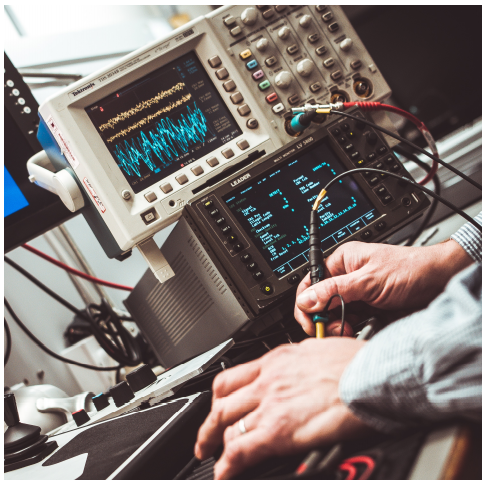
\includegraphics[scale=0.9]{portada.png}
\end{figure}

\hspace{1cm}
\begin{tabular}{|c| p{122mm}|}
	\hline
	\multirow{4}{50mm}{\\ \centering \large Apellidos y nombres}	 &  \\  
	& Alfaro Domínguez Rodrigo  \\  \cline{2-2}
	&  \\  
	& Barrera Peña Víctor Miguel \\  \cline{2-2}
	&  \\  
	& Villeda Hernández Erick Ricardo \\ 
	\hline
\end{tabular}
\begin{tabular}{|p{50mm} | c | p{108mm}|}
	Grpo: & 4 & \multirow{2}{100mm}{Profesor: M.I Lauro Fernando Vazquez Alberto } \\ \cline{1-2}
	Brigada: & 1 & \\ \hline
	Semestre: & 2021-1 & Fecha de ejecución: 29/09/2020 \\ \hline
\end{tabular}

\section{Previo}

\setlength{\parindent}{25pt}

\paragraph{1) Físicamente, ¿qué es una señal? \\
}

Una perturbación en un medio físico que puede transmitirnos información

\paragraph{2) ¿A qué se refiere el término sistema?}

 Un sistema es una interconexión de componentes y dispositivos por medio  del  cual  una  señal  de  entrada  es  transformada  para  producir  una  señal  de  salida


\paragraph{3) ¿Qué relación existe entre las señales y los sistemas? y ¿Cuál es la importancia de su análisis?}

La relación entre señales y sistemas es que los sistemas son usados para transformar una señal de entra y obtener una señal de salida, es decir, los sistemas son capaces de procesar y analizar las señales para obtener un resultado previa mente pensado

\paragraph{4) ¿Qué es un generador de funciones? y ¿Cuáles son las principales características de éstos?}

Un generador de funciones es una \textit{fuente de señales} con la capacidad de formar ondas. Los generadores de funciones tienen la capacidad de formar ondas senoidales, cuadradas y triangulares dentro de un cierto rango de frecuencias, normalmente entre 0.01Hz y 1 MHz.	
\newline

\noindent Sus características principales son:
\begin{center}
	\begin{table}[htbp]
		\centering
		\begin{tabular}{|c|c|}
			\hline
			\textbf{Característica} & 					\textbf{Medida}\\	\hline
			Rango de Frecuencia & 0.1 Hz a 11 MHz	\\	\hline
			Exactitud & $\pm 5\%$ de la escala del rango\\ & de frecuencia\\	\hline
			Sensibilidad & 1 Hz a 50 MHz\\		\hline
			Graduación & 1 a 11 calibrado \\ & 0.1 a 1 sin calibrar\\	\hline
			Impendencia de salida principal & 50 ohm $\pm 10\%$ \\	\hline
			Impendancia & 1 M ohm en paralelo con 40 pF\\ \hline
			Resolución & Modo de frecuencua: 1 Hz,10 Hz,1 kHz \\ & Modo de periodo: 1 ms\\ \hline
			Compensación de DC & $<-10$ V a $>+ 10$ V\\
			\hline
			Distorsión de onda sinoidal & $<1\%$ de 10 Hz a 100 kHz \\ & -30dB en todas las demás frecuencias\\	\hline
			Linealidad de la onda Trinagular & 0.1 Hz a 100 Hz > o >= $99\%$ \\ & 100 kHz a 1 MHz > o >= $97\%$\\ \hline
			Transición de tiempo de la onda cuadrada & $<$= a 25ns de cambio de \\ & subida a bajada\\ \hline
			Aberraciones de onda cuadrada & $<= 4\%$ pico a pico\\ \hline
			Tiempo de subida / bajada de salida & $<$ 25 ns \\ TTL de sincronización & \\ \hline
			Dimensiones (H x W x D) & 100mm X 240mm X 230mm\\	\hline
			Peso & 3.0.kg\\ \hline
		\end{tabular}
		\newline 
	\end{table}
\end{center}


\paragraph{5) ¿Qué es un osciloscopio? y ¿Cuáles son las principales características de éste?}

El osciloscopio es un \textit{instrumento que permite visualizar ondas generadas por una corriente eléctrica}. Al mostrarse la onde en la pantalla, esta se gráfica en un plano cartesiano donde el eje X es el tiempo y el eje Y es la amplitud de la onda. De esta forma podemos observar las variaciones en la corriente eléctrica a lo largo del tiempo

\begin{itemize}
	\item Ancho de Banda: Este parámetro determina la frecuencia máxima de la señal a capturar y analizar. Mientras más se acerque la frecuencia al límite del ancho de banda el osciloscopio pierde exactitud. Ancho de banda = frecuencia x 5. El ancho de banda se mide en Hz.
	\item Exactitud de ganancia de DC vertical:  Dado que los osciloscopios no están diseñados para utilizarse en lugar de multímetros digitales, es probable que sus elementos de voltaje no sean tan precisos. Por lo tanto, se recomienda a los usuarios de osciloscopios que sean conscientes de la precisión de la medición realizada al medir la amplitud de la señal.
	\item Resolución: Determina la medida más grande que puede realizar el osciloscopio sin la necesidad de recortar la forma de la onda.
	\item Rango de Muestras: Hace referencia al número de muestras que puede manejar el osciloscopio por segundo. Se obtiene el valor de dicho parámetro al multiplicar la frecuencia por 2.5
	\item Tamaño de Memoria: Nos muestra el número de muestras que el osciloscopio puede guardar para su posterior procesamiento.
	\item Tiempo de subida: Se refiere a la habilidad del instrumento de captar la subida y bajada de las señales. Este parámetro es muy importante a la hora de trabajar con señales cuadradas ya que una señal puede variar de 0V a 5V en ns.
	\item Canales: un osciloscopio tiene entre 2 y 4 canales a través de los cuales se puede monitorear una señal. El número de canales hace referencia al número de señales que se pueden monitorear simultáneamente.
	\item Disparador: El disparador de un osciloscopio es el mecanismo a través del cual un osciloscopio puede reconocer un atributo específico de la señal monitoreada. Gracias a este atributo se puede generar sincronicidad entre el osciloscopio y la señar recibida.
\end{itemize}

Ejemplo de las especificaciones del osciloscopio PicoScope 5000 Series.
\newline
\newline
\begin{center}
	\begin{table}[htbp]
		\centering
		\begin{tabular}{|c|c|}
			\hline
			\textbf{Característica} & 					\textbf{Medida}\\	\hline
			Ancho de Banda & 60 MHz a 200 MHz \\ \hline
			Canales & 2 a 4 \\ \hline
			Tiempo de subida & 3.5 ns a 5.8 ns \\ \hline
			Rango de Muestras & 125 MS/s a 1 GS/s Depende del número de \\ & canales usado \\ \hline
			Exactitud de ganancia de DC vertical & $\pm 1\%$ de la escala total \\ \hline
		\end{tabular}
		\newline 
	\end{table}
\end{center}

\paragraph{6) En ingeniería, ¿Cuáles son las principales señales de prueba?,\\ mencione dos ejemplos donde se empleen dichas señaales haciendo énfasis en la aplicación.} 

En la ingeniería, las señales principales que se utilizan son la escalón, rampa, parábola, senoidales e impulso. Esto debido a su simplicidad ya que facilita el análisis matemático; además tambien son sencillas de trabajar al momento de realizar experimentos prácticos y/o simulaciones en algunos programas.

\begin{figure}[h]
	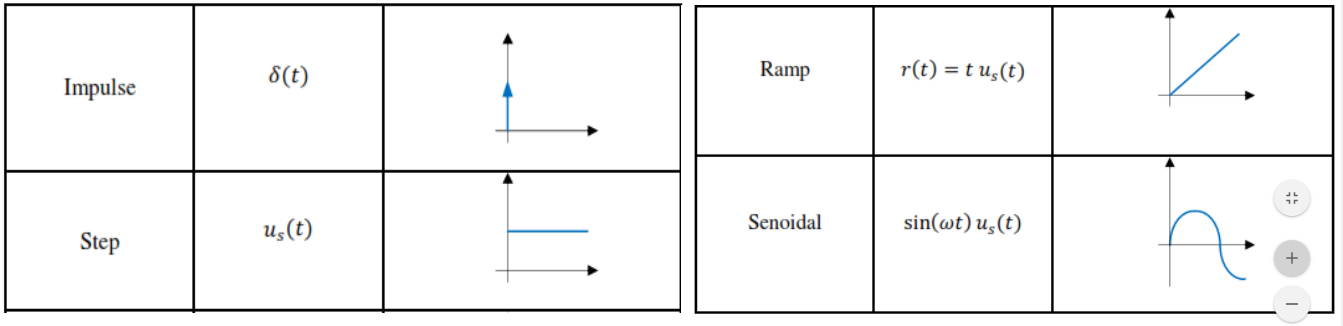
\includegraphics[scale=0.33]{sen}
	\centering
\end{figure}

\textbf{Ejemplo 1:}
La función escalón unitario, es una función continua cuyo valor es 0 para cualquier argumento negativo, y 1 para cualquier argumento positivo. Tiene diversas aplicaciones en la rama de la ingeniería, pero un uso frecuente se le da, es en la ingeniería de control y procesamiento de señales, ya que está representa una señal que se enciende en un tiempo específico, y se queda prendida indefinidamente. Por ejemplo una fuerza externa que actúa sobre un sistema mecánico o una tensión eléctrica aplicada a un circuito, puede tener que suspenderse después de cierto tiempo. \\

\textbf{Ejemplo 2:}
Otra señal frecuentemente utilizada en la rama de la ingeniería es la señal senoidal.  Un claro ejemplo de ello sería en el estudio de fenómenos periódicos como el sonido o la corriente eléctrica. La mayor parte de las aplicaciones prácticas de electricidad tienen que ver con corrientes eléctricas. Por ejemplo la batería de una luz de destellos suministra corriente al filamento de la bombilla cuando el interruptor se conectan. Aquí se puede apreciar el estudio de las señales senoidales.\\

\paragraph{7) ¿Cuáles son las principales caracter´ısticas de las siguientes operaciones de señales? }

\begin{itemize}
	\item Suma y resta
	\item Derivar e integrar.
	\item Escalonamiento y amplitud
\end{itemize}

\textbf{Suma y resta:}
La suma de dos señales siempre debe realizarse punto por punto es decir para cada valor de t se deben sumar los valores de las señales, respetando el signo que tienen cada una. En el caso particular de que una de las señales sea constante, el resultado se obtendrá de desplazar verticalmente a la otra señal tantas unidades como diga la constante, respetando su signo. A la señal resultante se le llama componente continua.
\begin{figure}[h]
	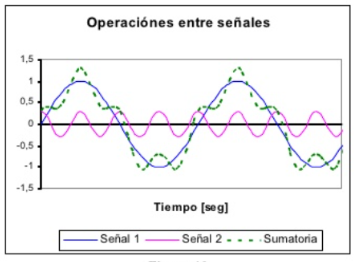
\includegraphics[scale=0.6]{S}
	\centering
\end{figure}

La resta de señales debe realizarse punto por punto. No obstante puede entenderse como una doble operación: primero invertir o multiplicar por -1 a la segunda señal; luego realizar la suma de ambas señales. Algo muy importante que se debe tener en cuenta al realizar una multiplicación de una señal por una constante es que siempre debe realizarse punto por punto. En este caso particular, el resultado de la misma señal variante aumentada en sus valores máximos y mínimos tantas veces como diga la constante. Si la constante es negativa el resultado inmediato es observar a la señal variante invertida respecto al eje tiempo.

\begin{figure}[h]
	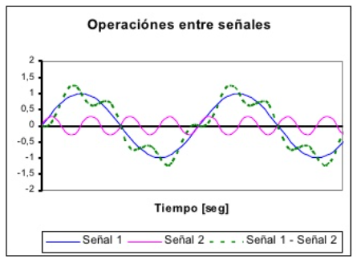
\includegraphics[scale=0.6]{R}
	\centering
\end{figure}

\textbf{Derivación e integración:}
La derivación de señales es muy usada en el modelado de sistemas, la podemos interpretar como la velocidad de cambio de la señal. Gráficamente representa su pendiente. Para el modelado de muchos sistemas se usan ecuaciones diferenciales, definidas como:

\[
\sum_{k=0}^{N}a_{k} \frac{d^{k}y(t)}{dt^{k}}=\sum_{k=0}^{M}b_{k} \frac{d^{k}x(t)}{dt^{k}}
\]

Algunos ejemplos de su utilización serían:
\begin{itemize}
	\item Respuesta de un circuito RC.
	\item Movimiento de un vehículo sujeto a entradas de aceleración y fuerzas de fricción.
\end{itemize}
A partir de una expresión para x(t) en función de señales elementales se puede obtener su derivada mediante el uso de las siguientes relaciones:

\[
\frac{dr(t)}{dt} = u(t)
\]

\[
\frac{du(t)}{dt} = \delta(t)
\]

\begin{figure}[h]
	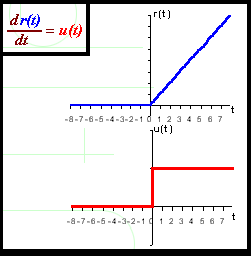
\includegraphics[scale=0.55]{3}
	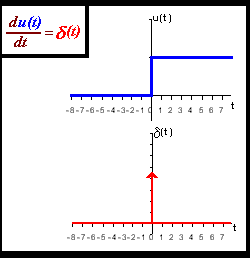
\includegraphics[scale=0.55]{4}
	\centering
\end{figure}

La integración de señales es una operación muy usada en comunicaciones, análisis espectral, etc., representando gráficamente el área acumulada bajo la curva que define la señal.
Las señales fundamentales, rampa y escalón,  están relacionadas por medio de las siguientes integrales:

\[
\int_{-\infty}^{t} \! u(\tau)  \,d\tau = r(t)
\]

\[
\int_{-\infty}^{t} \! \delta(\tau)  \,d\tau = u(t)
\]

\begin{figure}[h]
	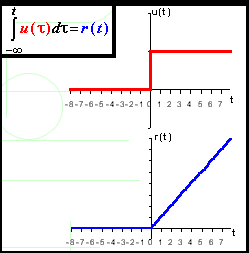
\includegraphics[scale=0.55]{1}
	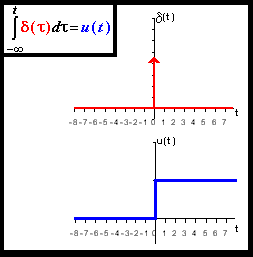
\includegraphics[scale=0.55]{2}
	\centering
\end{figure}

\textbf{Escalamiento de amplitud:}
El escalonamiento de amplitud es la transformación funcional más sencilla esta transformación está representada por la siguiente notación: 
Para cualquier valor de t, la transformación multiplica el valor producido de x(t) por A. 
A puede ser cualquier constante.
Un ejemplo de un dispositivo que realiza el escalonamiento de amplitud es un amplificador electrónico.


\section{Bibliografía:}

\begin{itemize}
	\item Instituto tecnológico de la Laguna, (s.f.), "Generador de funciones" obtenido electrónicamente el día 26 de septiembre del 2020 a las 18:57 de \url{http://www.itlalaguna.edu.mx/
		academico/carreras/sistemas/Ecabas/ecabaspdf/GENERADOR\%20DE\%20FUNCIONES.pdf}
	\item Tectronik Inc, (s.f), "Function generator, general description and specifications", obtenido electrónicamente el día 26 de sepriembte del 2020 a las 19:00 de \url{http://www.ceen.unomaha.edu/labmaster/RM305,311/PAGES/FNCTGEN_GEN_DSRP_SPC.htm}
	\item Electronics Notes, (s.f.), "What is an Oscilloscope: basics \& fundamentals", recuperado electrónicamente el día 26 de septiembre del 2020 a las 19:09 de \url{https://www.electronics-notes.com/articles/test-methods/oscilloscope/scope-basics.php}
	\item Test and Measurement, 2016, "Important oscilloscope specification", recuperado electrónicamente el día 26 de septiembre del 2020 a las 20:01 de \\ \url{https://www.testandmeasurementtips.com/important-oscilloscope-specification/}
	\item Sin autor, sin fecha, "Oscilloscope specifications", recuperado electrónicamente el día 26 de septiembre del 2020 a las 20:09 de \url{https://techexplorations.com/guides/tools/oscilloscope/specifications/}
	\item Sin autor, sin fecha, "PicoScope® 5000 Series", recuperado electrónicamente el 26 de septiembre del 2020 a las 21:44 de \url{https://www.picotech.com/oscilloscope/5000/picoscope-5000-specifications}
	\item 	Cervantes, J.(13 de marzo de 2019).\textit{ Matematicas V (Unidad 3)}. Blogspot. Recuperado el 26 de septiembre de 2020 de http://maunidad3.blogspot.com/2011/05/35-funcion-escalon-unitario.html\\
	
	\item Muno, E.(2 de agosto de 2014).\textit{ Señales y sistemas}. Slideplayer. Recuperado el 26 de septiembre de 2020 de https://slideplayer.es/slide/1487132/\\
	
	\item Rodríguez, R.(4 de julio de 2010).\textit{ Características de las Señales}. Slideshare. Recuperado el 26 de septiembre de 2020 de https://es.slideshare.net/5transmisiondedatos/caractersticas-de-las-seales\\
	
	\item Villamil, S.(27 de abril de 2018).\textit{ Derivación de señales}.Unet. Recuperado el 26 de septiembre de 2020 de http://www.unet.edu.ve/aula10c/Asenales/Unid01/cuarto06.htm
	
	\item Bibliografía: Alicia Denis, (s.f.), Señales y Sistemas, recuperado electrónicamente el día 28 de septiembre del 2020 a las 21:00 de 
\end{itemize}

\end{document}




